\documentclass[9pt]{extarticle}
\usepackage[margin=0.7cm]{geometry}
\usepackage[UKenglish]{babel}
\usepackage{parallel,enumitem}
\usepackage{multicol}
\setlength{\columnsep}{0.7cm}
\setlength{\columnseprule}{0.5pt}
\usepackage{amssymb}
\usepackage{amsmath}
\usepackage{bm}
\usepackage{graphicx}
\graphicspath{{./pics/}}
\usepackage{physics}

%% vectors and matrices
\renewcommand{\v}[1]{{\bm #1}}
\renewcommand{\dv}[1]{\dot{\bm{#1}}}
\newcommand{\ddv}[1]{\ddot{\bm{#1}}}
\newcommand{\hv}[1]{\hat{\bm{#1}}}
\newcommand{\m}[1]{[ #1 ]}
\renewcommand{\t}[1]{\widetilde{\bm{#1}}}
\newcommand{\bfit}[1]{\textbf{\textit{#1}}}

%% differential and integral operators
\renewcommand{\d}{\text{d}}
\renewcommand{\dd}[2]{\frac{\d #1}{\d #2}}
\newcommand{\ddd}[2]{\frac{\d^2 #1}{\d #2^2}}
\newcommand{\ddt}[1]{\frac{\d #1}{\d t}}
\newcommand{\dddt}[1]{\frac{\d^2 #1}{\d t^2}}
\newcommand{\pd}[2]{\frac{\partial #1}{\partial #2}}
\newcommand{\pdd}[2]{\frac{\partial^2 #1}{\partial #2^2}}
\renewcommand{\grad}{\boldsymbol \nabla} 
\renewcommand{\div}{\boldsymbol \nabla \cdot}
\renewcommand{\curl}{\boldsymbol \nabla \times}
\newcommand{\lap}{\nabla^2}

%% constants
\newcommand{\eo}{\epsilon_0}
\newcommand{\muo}{\mu_0}

%% statistics
\newcommand{\E}{\text{E}}
\newcommand{\Var}{\text{Var}}
\newcommand{\SD}{\text{SD}}
\newcommand{\SE}{\text{SE}}
\newcommand{\Cov}{\text{Cov}}
\newcommand{\Cor}{\text{Cor}}
\renewcommand{\P}{\text{P}}
\newcommand{\Bias}{\text{Bias}}

\begin{document}

\setlength{\parindent}{0pt}

{\huge \bf problem set} 

\noindent \hrulefill

\begin{multicols*}{2}

{\bf \LARGE I --- Mutual Inductance of Two Loops} \\

{\it Griffiths 7.22} \\ 

A small loop of wire (radius $a$) is held a distance $z$ above a large loop (radius $b$), as shown in the figure below. The planes of the two loops are parallel, and perpendicular to the common axis.    

\begin{center}
	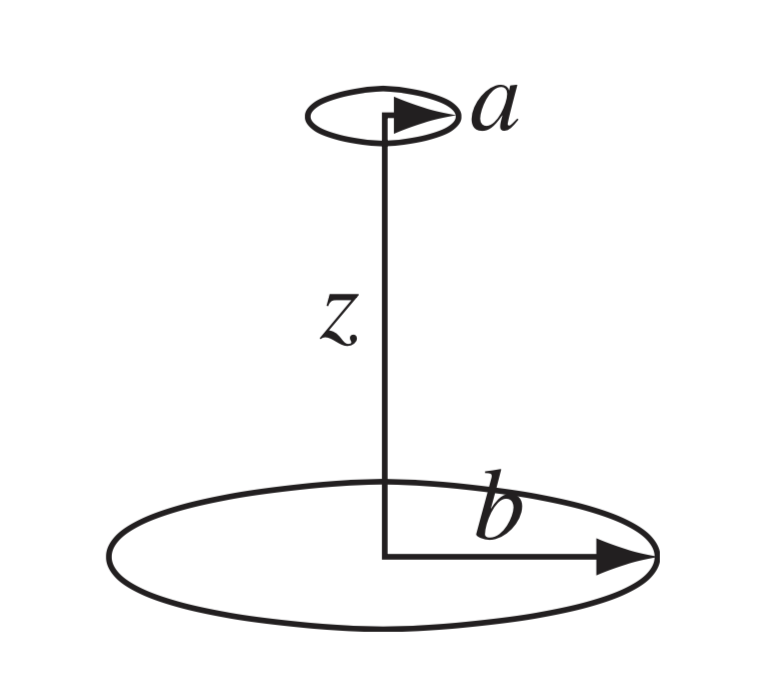
\includegraphics[scale=0.2]{ps8-pic1.png}
\end{center}

{\bf \Large a.} Suppose current $I$ flows in the big loop.  Find the flux through the little loop.  Note the little loop is so small that you may consider the field of the big loop to be essentially constant. \\ 

{\bfit{Solution}} \\ 

The magnetic field a distance $z$ above a loop of radius $b$ is given by:

$$\v B = \frac{\muo I}{2} \frac{b^2}{(b^2+z^2)^{3/2}} \hv z$$ \ 

The flux through the small loop is:

$$\v \Phi_B = \v B \cdot A = \frac{\muo I}{2} \frac{\pi a^2 b^2}{(b^2+z^2)^{3/2}}$$ \ 





\dotfill 

\hfill 

{\Large \bf b.} Suppose current $I$ flows in the little loop. Find the flux through the big loop. Note the little loop is so small that you may treat it as a magnetic dipole. \\ 

{\bfit{Solution}} \\ 

The field in this case is given by:

$$\v B = \div A = \frac{\muo}{4\pi} \frac{m}{r^3} (2\cos\theta \hv r + \sin\theta \hv \theta)$$ \ 

where $m = I\pi a^2$. To find the flux through the big loop, integrate as follows:

$$\v \Phi_B =  \int \v B \cdot \d \v a = \frac{\muo I}{4\pi} \frac{\pi a^2}{r^3} \int 2\cos\theta r^2\sin\theta \d \theta \d \phi$$  

$$= \frac{\muo I}{2} \frac{\pi a^2 b^2}{(b^2+z^2)^{3/2}}$$ \ 

i.e. the flux is the same as in part a. \\ 





\dotfill 

\hfill 

{\Large \bf c.} Find the mutual inductances, and confirm that $M_{12} = M_{21}$. \\  

{\bfit{Solution}} \\ 

Since $\v \Phi_1 = M_{12} I_2$ and $\v \Phi_2 = M_{21} I_1$, it follows that:

$$M_{12} = \frac{\muo \pi a^2 b^2}{2(b^2+z^2)^{3/2}} = M_{21}$$ \ 




\hrulefill 

\columnbreak 

{\LARGE \bf II --- Loop Around a Solenoid} \\ 

Consider a single loop of wire wrapped around the outside of an infinite solenoid, as shown in the figure below. The solenoid is circular in cross section with radius $R$ and $n$ coils per unit length. The single loop is irregular in shape, but (of course) larger than the  solenoid.  Also, none of the  answers require the  loop to be oriented parallel  to the solenoid. For simplicity, assume the loop is contained in one plane. 

\begin{center}
	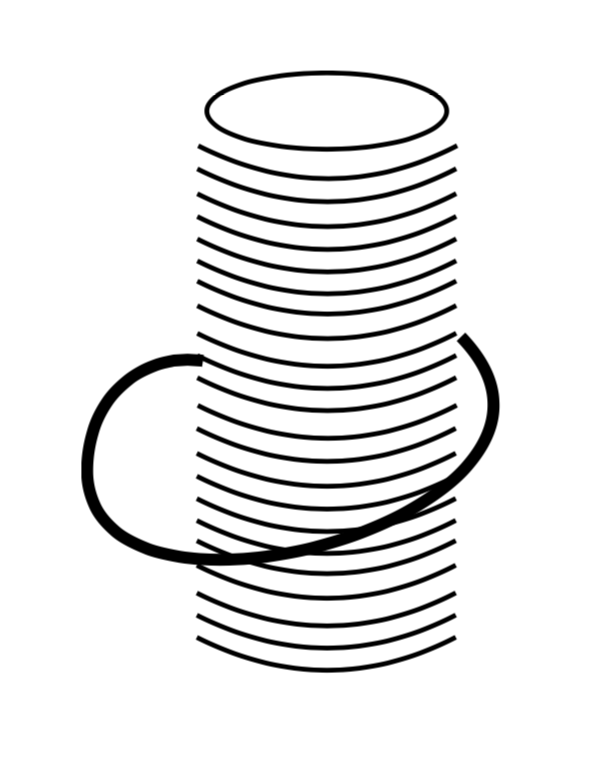
\includegraphics[scale=0.3]{ps8-pic2.png}
\end{center}

{\Large \bf a.} Find the mutual inductance $M$ between the loop and the solenoid. \\ 

{\bfit{Solution}} 

Since the number of loops around the solenoid is 1, the mutual inductance between the loop and the solenoid is:

$$M = \muo nA$$ \ 



\dotfill 

\hfill 

{\Large \bf b.} Suppose now that the loop goees around the solenoid twice. Again, find the mutual inductance $M$. \\ 

{\bfit{Solution}} \\ 

Since now the number of loops around the solenoid  is 2, the mutual  inductance is:

$$M = 2\muo nA$$ \ 




\dotfill 

\hfill 

{\Large \bf c.} Find the self-inductance per unit length of the infinite solenoid, all by itself. Now check that the units of your answer work out correctly. Begin by expressing the units of $\muo$ in terms of Henries. \\ 

{\bfit{Solution}} \\ 

$$\varepsilon = -\ddt{(N\muo n IA)} =  -nl \muo  n A \ddt I  = -\L \ddt I$$ \ 

Thus the self inductance $L$ is:

$$L = \muo n^2 lA$$ \ 

And, the self inductance per unit length is:

$$\frac Ll = \muo n^2 A$$ \ 

The units on the LHS and RHS are both kgm$^2$s$^{-2}$A$^{-2}$. \\ 






\hrulefill 

\hfill 

{\LARGE \bf III --- Back EMF} \\ 

{\it Griffiths 7.26} \\ 

An alternating current $I(t) = I_0\cos\omega t$, which  has  amplitude 0.5 A and frequency 60 Hz, flows down a straight wire, which runs along the axis of a toroidal coil with rectangular cross section,  of inner radius 1 cm, outer radius 2cm, height 1 cm, and 1000 turns. The coil is connected to a 500 $\Omega$ resistor. \\ 

{\bf \Large a.} In  the quasistatic approximation, what emf is induced in the toroid? Find the current, $I_R(t)$, in the resistor. \\ 

{\bfit{Solution}} \\ 

In the quasistatic approximation, the field is:

$$\v B = \frac{\muo}{2\pi s} \hv \phi$$ \ 

The flux through one turn of coil is:

$$\v \Phi_B (\text{one turn}) = \frac{\muo I}{2\pi} \int_a^b \frac 1s h \d s = \frac{\muo I h}{2\pi} \ln \big( \tfrac ba \big)$$ \ 

The flux through $N$ turns of coil is thus:

$$\v \Phi_B = \frac{\muo Nh}{2\pi} \ln \big( \tfrac ba \big) I_0 \cos\omega t$$ \

By Faraday's law, the induced emf is:

$$\varepsilon = -\ddt \Phi = \frac{\muo Nh}{2\pi} \ln \big( \tfrac ba \big) I_0 \omega\sin\omega t$$ \

Substituting the values above:

$$\varepsilon = \frac{(4\pi \cdot 10^{-7})(10^3)(10^{-2})}{2\pi} \ln(2) (0.5) (2\pi \cdot 60) \sin\omega t$$

$$= 2.61 \cdot 10^{-4} \sin\omega t \;\; \text V$$ \ 

The current in the resistor, by Ohm's law, is:

$$I_R = \frac \varepsilon R = \frac{2.61 \cdot 10^{-4}}{500}\sin\omega t =  5.21 \cdot 10^{-7} \sin\omega t\;\; \text A$$ \  




\dotfill 

\hfill 

{\Large \bf b.} Calculate the back emf in the coil, due to the current $I_R(t)$. What is the ratio of the amplitudes of this back emf and the ``direct" emf in part a? \\ 

{\bfit{Solution}} \\ 

The back emf, $\varepsilon_b$, is given by $\varepsilon_b = -L \ddt{I_R}$, where in this case the self-inductance, $L$, is:

$$L = \frac{\muo N^2 h}{2\pi} \ln \big( \tfrac ba \big) = 1.4 \cdot 10^{-3} \;\; \text H$$ \ 

Thus the back emf is:

$$\varepsilon_b = -(1.4 \cdot 10^{-3}) (5.21 \cdot 10^{-7} \omega\cos\omega t) = -2.78 \cdot 10^{-7}\cos\omega t\;\; \text V$$ \ 

The ratio of amplitudes of the back emf and the ``direct" emf is:

$$\frac{2.78 \cdot 10^{-7}}{2.61 \cdot 10^{-4}} = 1.07  \cdot 10^{-3}$$ \







\hrulefill 

\hfill 

{\LARGE \bf IV --- Energy Stored in a Rotating Cylinder} \\ 

{\it Griffiths 7.33} \\ 

An infinite cylinder of radius $R$ carries a uniform surface charge $\sigma$. We propose to set it spinning about its axis, at a final angular velocity $\omega_f$. How much work will this take, per unit length? Do it two ways, and compare your answers: \\ 

{\Large \bf a.} Find the magnetic field and the induced electric field (in the quasistatic  approximation), inside and outside the cylinder, in terms of $\omega,  \dot\omega$, and $s$ (the distance from the axis). Calculate the torque you must exert, and from that obtain the work  done per unit length ($W = \int N\d\phi$). \\ 

{\bfit{Solution}} \\ 

The magnetic field for a solenoid is:

$$
\v B = 
\begin{cases}
	\muo \sigma\omega R \hv z & s < R \\ 
	0 & s > R
\end{cases}
$$ \ 

The electric field is:

$$
\v E = 
\begin{cases}
	 -\frac{Rs}{2} \muo \sigma \dot\omega \hv \phi & s < R \\
	 \\ 
	 -\frac{R^3}{2s} \muo \sigma \dot\omega \hv \phi & s > R
\end{cases}
$$ \ 

When $s=R$, the eleectric field is:

$$\v E = -\frac 12 \muo R^2 \sigma \dot\omega \hv \phi \hspace{1cm} s=R$$ \ 

Thus the torque on a length of cylinder $l$ is:

$$\v \tau = -R\sigma 2\pi Rl \cdot \tfrac 12 \muo R^2 \sigma \dot\omega \hv z = -\pi \muo R^4 \sigma^2 \dot\omega l \hv z$$ \ 

The work  done per unit length is:

$$\frac Wl = -\pi \muo \sigma^2 R^4 \int \ddt\omega \d \phi = -\frac{\muo  \pi}{2} (\sigma \omega_f R^2)^2$$ \ 




\dotfill 

\hfill 

{\Large \bf b.} Use eq. 7.35 to  determine the energy stored in the resulting magnetic field. \\ 

{\bfit{Solution}} \\ 

Equation 7.35:

$$W = \frac{1}{2\muo} \int_{\text{all space}} B^2 \d V$$ \ 

Since the magnetic field is uniform inside the solenoid, and zero outside the solenoid:

$$W = \frac{1}{2\muo} B^2 \pi R^2 l$$ \ 

Thus the work per unit length is:

$$\frac Wl = \frac{1}{2\muo} (\muo \sigma\omega_f R)^2 \pi R^2$$ 

$$= \frac{\muo \pi}{2} (\sigma\omega_f R^2)^2$$ \ 






\hrulefill 

\hfill 

{\LARGE \bf V --- Magnetic Field in an Alternating Capacitor} \\ 

Consider a parallel-plate capacitor in an RLC circuit such that it experiences alternating current. The plates are circles of radius $R$ spaced a distance $d$ apart. Assume the surface charge on the plates is uniform and given as a function of time as $\sigma(t) = \sigma_0\sin\omega t$.  \\ 

{\Large \bf a.} Find the electric fieeld beetween the plates as a function of time. Assume the spacing $d$ between the plates is much smaller than the dimensions of the plates $ d \ll R$ such that when computing the electric field you can assume the limit where the plates are infinitely large. \\ 

{\bfit{Solution}}  \\ 

The electric field as a function of time is simply: 

$$\v E(t) = \frac{\sigma(t)}{\eo} = \frac{\sigma_0}{\eo} \sin\omega t$$ \ 




\dotfill 

\hfill 

{\Large \bf b.} Find the magnetic field between the plates as a function  of time. Approximate the electric field as being nonzero only between the plates, i.e. $\v E (s>R) = 0$.  \\  

{\bfit{Solution}}  \\ 

The magnetic field as a function of time is:

$$\v B(t) = \tfrac 12 \muo \sigma \omega r \cos\omega t$$ \ 

where $r$ is the distance from the center of the plates. \\ 







\hrulefill 

\hfill 

{\LARGE \bf VI --- Magnetic Monopoles} \\ 

{\Large \bf a.} {\it Griffiths 7.38:} Assuming that ``Coulomb's law" for magnetic charges ($q_m$) reads:

$$\v F = \frac{\muo}{4\pi} \frac{q_{m_1} q_{m_2}}{r^2} \hv r$$ \ 

work out the force law for a monopole $q_m$ moving with  velocity $\v v$ through electric and magnetic fields $\v E$ and $\v B$. \\ 

{\bfit{Solution}} \\ 

For a monopole, $\div \v B = \muo \rho_m$, and thus its field would be :

$$\v B = \frac{\muo}{4\pi} \frac{q_m}{r^2} \hv r$$ \ 

This gives the following force law:

$$\v F = q_m \big( \v B - \tfrac{1}{c^2} \v v \times \v E \big)$$ \ 





\dotfill 

\hfill 

{\Large \bf b.} {\it Griffiths 7.64:} \\ 

{\bf i.} Show that Maxwell's equatoins  with magnetic charge (eq 7.44) are invariant under the duality transformation:

$$\v E' = \v E\cos\alpha + c\v B\sin\alpha$$
$$c\v B' = c\v B\cos\alpha - \v E\sin\alpha$$
$$cq_e' = cq_e \cos\alpha + q_m\sin\alpha$$
$$q_m' = q_m\cos\alpha  -  cq_e\sin\alpha$$ \ 

where $c = 1/\sqrt{\eo\muo}$ and $\alpha$ is an arbitrary rotation angle in ``$\v E/\v B$-space". Charge and current densities transform in the same way as $q_e$ and $q_m$. This means, in particular, that if you know the fields produced by a configuration of electric charge, you can immediately (using $\alpha = 90^o$) write down the fields produced by the corresponding arrangement of magnetic charge. \\ 

{\bfit{Solution}} \\ 

Checking each of the Maxwell equations:

$$\div \v E' = (\div \v E) \cos\alpha + c(\div \v B)\sin\alpha = \frac 1 \eo \rho_e \cos\alpha + c\muo \rho_m\sin\alpha$$

$$= \frac 1\eo \bigg( \rho_e \cos\alpha + \frac 1c \rho_m\sin\alpha \bigg) = \frac 1\eo \rho_e'$$ 
q.e.d. \\ 

$$\div \v B' = (\div \v B)\cos\alpha - \frac 1c (\div \v E)\sin\alpha = \muo \rho_m\cos\alpha - \frac{1}{c\eo}\rho_e\sin\alpha$$

$$= \muo(\rho_m \cos\alpha - c\rho_e\sin\alpha) = \muo\rho_m'$$ \ 

q.e.d. \\ 

$$\curl \v E' = (\curl \v E)\cos\alpha + c(\curl \v B)\sin\alpha$$

$$= \bigg(-\muo \v J_m - \pd{\v B}{t} \bigg) \cos\alpha + c\bigg( \muo \v J_e + \muo \eo \pd{\v E}{t} \bigg) \sin\alpha$$

$$= \muo \v J_m' - \pd{\v B'}{t}$$ 

q.e.d. \\ 

$$\curl \v B' = (\curl \v B)\cos\alpha - \frac 1c (\curl \v E)\sin\alpha$$

$$= \bigg(\muo J_e + \muo\eo \pd{\v E}{t} \bigg) \cos\alpha - \frac 1c \bigg(-\muo \v J_m -\pd{\v B}{t} \bigg) \sin\alpha$$ 

$$= \muo \v J_e' + \muo\eo \pd{\v E'}{t}$$

q.e.d. \\ 

Thus, we can conclude that Maxwell's equations with magnetic charges are invariant under the duality transformation. \\ 




\dotfill 

\hfill 

{\bf ii.} Show that the force law (prob 7.38):

$$\v F = q_e(\v E + \v v \times \v B) + q_m \big( \v B - \tfrac{1}{c^2}\v v \times \v E \big)$$ \ 

is also invariant under the duality transformation. \\ 

{\bfit{Solution}} \\ 

From problem 7.38:

$$\v F' = q_e'(\v E' + \v v \times \v B') + q_m'(\v B' - \frac{1}{c^2} \v v \times \v E')$$

$$= \bigg(q_e\cos\alpha + \frac 1c q_m  \sin\alpha \bigg) \bigg[ (\v E \cos\alpha + c\v B \sin\alpha) + \v v \times \bigg( \v B\cos\alpha - \frac 1c \v E\sin\alpha \bigg) \bigg]$$

$$+ \bigg( q_m \cos\alpha - cq_e \sin\alpha \bigg) \bigg[ \bigg( \v B \cos\alpha - \frac 1c \v  E\sin\alpha \bigg) - \frac{1}{c^2} \v v \times (\v E\cos\alpha + c \v B\sin\alpha)  \bigg]$$ \ 

$$= q_e (\v E + \v v \times \v B) + q_m \bigg( \v B - \frac{1}{c^2} \v v \times \v E \bigg) = \v F$$ \ 

Thus, the force law for a monopole is also invariant under the duality transformation. 

\end{multicols*}

\end{document}
